\documentclass[12pt,a4paper]{article}
\usepackage{charter}
%\usepackage[latin1]{inputenc}
\usepackage[left=1.50cm, right=1.50cm, top=1.20cm]{geometry}
\usepackage{amsmath}
\usepackage{amsfonts}
\usepackage{amssymb}
\usepackage{graphicx}
\usepackage{textcomp}
\renewcommand{\baselinestretch}{1.5}
\usepackage{listings}
\usepackage{xcolor}
\definecolor{listinggray}{gray}{0.9}
\definecolor{lbcolor}{rgb}{0.9,0.9,0.9}
\usepackage{float}
\usepackage{CJKutf8}
\usepackage{textcomp}
\usepackage{hyperref}
%\lstset{
%	backgroundcolor=\color{lbcolor},
%	tabsize=4,    
%	%   rulecolor=,
%	language=[GNU]C++,
%	basicstyle=\scriptsize,
%	upquote=true,
%	aboveskip={1.5\baselineskip},
%	columns=fixed,
%	showstringspaces=false,
%	extendedchars=false,
%	breaklines=true,
%	prebreak = \raisebox{0ex}[0ex][0ex]{\ensuremath{\hookleftarrow}},
%	frame=single,
%	numbers=left,
%	showtabs=false,
%	showspaces=false,
%	showstringspaces=false,
%	identifierstyle=\ttfamily,
%	keywordstyle=\color[rgb]{0,0,1},
%	commentstyle=\color[rgb]{0.026,0.112,0.095},
%	stringstyle=\color[rgb]{0.627,0.126,0.941},
%	numberstyle=\color[rgb]{0.205, 0.142, 0.73},
%	%        \lstdefinestyle{C++}{language=C++,style=numbers}?.
%}
%\lstset{
%	backgroundcolor=\color{lbcolor},
%	tabsize=4,
%	language=C++,
%	captionpos=b,
%	tabsize=3,
%	frame=lines,
%	numbers=left,
%	numberstyle=\tiny,
%	numbersep=5pt,
%	breaklines=true,
%	showstringspaces=false,
%	basicstyle=\footnotesize,
%	%  identifierstyle=\color{magenta},
%	keywordstyle=\color[rgb]{0,0,1},
%	commentstyle=\color{Darkgreen},
%	stringstyle=\color{red}
%}

\lstdefinestyle{customc}{
	belowcaptionskip=1\baselineskip,
	aboveskip={1.2\baselineskip},
	breaklines=true,
	frame=lines,
	numbers=left,
	xleftmargin=\parindent,
	language=C++,
	showstringspaces=false,
	basicstyle=\sffamily,%,\ttfamily,
	keywordstyle=\bfseries\color{green!40!black},
	commentstyle=\itshape\color{purple!40!black},
	identifierstyle=\color{blue},
	stringstyle=\color{orange},
	breaklines=true,
	postbreak=\raisebox{0ex}[0ex][0ex]{\ensuremath{\color{red}\hookrightarrow\space}}
}

\lstdefinestyle{customasm}{
	belowcaptionskip=1\baselineskip,
	frame=L,
	xleftmargin=\parindent,
	language=[x86masm]Assembler,
	basicstyle=\footnotesize\ttfamily,
	commentstyle=\itshape\color{purple!40!black},
}

\lstset{escapechar=@,style=customc}

\begin{document}
\section{Solution}
\subsection{60}
\begin{CJK}{UTF8}{gbsn}
这道题是让求出n个数字的第k个排列组合,由于其特殊性,我们不用将所有的排列组合的情况都求出来,然后返回其第k个,
我们可以只求出第k个排列组合即可,那么难点就在于如何知道数字的排列顺序,
首先我们要知道当n = 3时,其排列组合共有$3! = 6$种,当n = 4时,其排列组合共有$4! = 24$种,
我们就以n = 4, k = 17的情况来分析,所有排列组合情况如下:
\end{CJK}
\begin{center}
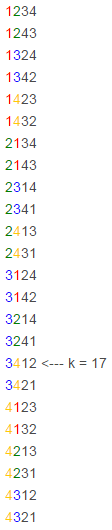
\includegraphics{0060.png}
\end{center}
\begin{CJK}{UTF8}{gbsn}
我们可以发现,每一位上1,2,3,4分别都出现了6次,当第一位上的数字确定了,后面三位上每个数字都出现了2次,当第二位也确定了,后面的数字都只出现了1次,当第三位确定了,那么第四位上的数字也只能出现一次,那么下面我们来看k = 17这种情况的每位数字如何确定,由于k = 17是转化为数组下标为16:
\par
最高位可取1,2,3,4中的一个,每个数字出现$3!= 6$次,所以k = 16的第一位数字的下标为$16 / 6 = 2$,即3被取出
\par
第二位此时从1,2,4中取一个,$k = 16$是此时的$k_1 = 16 \% (3!)$ = 4,而剩下的每个数字出现$2!= 2$次,所以第二数字的下标为$4 / 2 = 2$,即4被取出
\par
第三位此时从1,2中去一个,$k_1 = 4$是此时的$k_2 = 4 \% (2!) = 0$,而剩下的每个数字出现$1!= 1$次,所以第三个数字的下标为 $0 / 1 = 0$,即1被取出
\par
第四位是从2中取一个,$k_2 = 0$是此时的$k_3 = 0 \% (1!) = 0$,而剩下的每个数字出现$0!= 1$次,所以第四个数字的下标为$0 / 1= 0$,即2被取出
\par
那么我们就可以找出规律了
\end{CJK}
\par
$a_1 = k / (n - 1)!$
\par
$k_1 = k$
\par
$a_2 = k_1 / (n - 2)!$
\par
$k_2 = k_1 \% (n - 2)!$
\par
\dots
\par
$a_{n-1} = k_{n-2} / 1!$
\par
$k_{n-1} = k_{n-2} / 1!$
\par
$a_n = k_{n-1} / 0!$
\par
$k_n = k_{n-1} \% 0!$
\begin{lstlisting}
string getPermutation( int n, int k ) {
	string res;
	string num = "123456789";
	vector<int> f( n, 1 );
	for ( int i = 1; i < n; ++i ) f[i] = f[i - 1] * i;
	--k;
	for ( int i = n; i >= 1; --i ) {
		int j = k / f[i - 1];
		k %= f[i - 1];
		res.push_back( num[j] );
		num.erase( j, 1 );
	}
	return res;
}
\end{lstlisting}


\subsection{61}
\begin{enumerate}
\item
\begin{CJK}{UTF8}{gbsn}
这道旋转链表的题和之前那道 Rotate Array 旋转数组 很类似,但是比那道要难一些,因为链表的值不能通过下表来访问,只能一个一个的走,我刚开始拿到这题首先想到的就是用快慢指针来解,快指针先走k步,然后两个指针一起走,当快指针走到末尾时,慢指针的下一个位置是新的顺序的头结点,这样就可以旋转链表了,自信满满的写完程序,放到OJ上跑,以为能一次通过,结果跪在了各种特殊情况,首先一个就是当原链表为空时,直接返回NULL,还有就是当k大于链表长度和k远远大于链表长度时该如何处理,我们需要首先遍历一遍原链表得到链表长度n,然后k对n取余,这样k肯定小于n,就可以用上面的算法了
\end{CJK}
\begin{lstlisting}
ListNode *rotateRight( ListNode *head, int k ) {
	if ( !head ) return NULL;
	int n = 0;
	ListNode *cur = head;
	while ( cur ) {
		++n;
		cur = cur->next;
	}
	k %= n;
	ListNode *fast = head, *slow = head;
	for ( int i = 0; i < k; ++i ) {
		if ( fast ) fast = fast->next;
	}
	if ( !fast ) return head;
	while ( fast->next ) {
		fast = fast->next;
		slow = slow->next;
	}
	fast->next = head;
	fast = slow->next;
	slow->next = NULL;
	return fast;
}
\end{lstlisting}
\item
\begin{CJK}{UTF8}{gbsn}
这道题还有一种解法,跟上面的方法类似,但是不用快慢指针,一个指针就够了,
原理是先遍历整个链表获得链表长度n,然后此时把链表头和尾链接起来,
在往后走$n - k \% n$个节点就到达新链表的头结点前一个点,这时断开链表即可
\end{CJK}
\begin{lstlisting}
ListNode *rotateRight( ListNode *head, int k ) {
	if ( !head ) return NULL;
	int n = 1;
	ListNode *cur = head;
	while ( cur->next ) {
		++n;
		cur = cur->next;
	}
	cur->next = head;
	int m = n - k % n;
	for ( int i = 0; i < m; ++i ) {
		cur = cur->next;
	}
	ListNode *newhead = cur->next;
	cur->next = NULL;
	return newhead;
}
\end{lstlisting}
\end{enumerate}


\subsection{62}
\begin{CJK}{UTF8}{gbsn}
这道题让求所有不同的路径的个数,一开始还真把我难住了,因为之前好像没有遇到过这类的问题,所以感觉好像有种无从下手的感觉。
在网上找攻略之后才恍然大悟,原来这跟之前那道 Climbing Stairs 爬梯子问题 很类似,那道题是说可以每次能爬一格或两格,问到达顶部的所有不同爬法的个数。而这道题是每次可以向下走或者向右走,
求到达最右下角的所有不同走法的个数。那么跟爬梯子问题一样,我们需要用动态规划Dynamic Programming来解,
我们可以维护一个二维数组dp,其中dp[i][j]表示到当前位置不同的走法的个数,
然后可以得到递推式为: dp[i][j] = dp[i - 1][j] + dp[i][j - 1],
这里为了节省空间,我们使用一维数组dp,一行一行的刷新也可以,代码如下
\end{CJK}
\begin{lstlisting}
int uniquePaths( int m, int n ) {
	vector<int> dp( n, 1 );
	for ( int i = 1; i < m; ++i ) {
		for ( int j = 1; j < n; ++j ) {
			dp[j] += dp[j - 1];
		}
	}
	return dp[n - 1];
}
\end{lstlisting}

\subsection{63}
\begin{enumerate}
\item
\begin{CJK}{UTF8}{gbsn}
这道题是之前那道 Unique Paths 不同的路径 的延伸,在路径中加了一些障碍物,
还是用动态规划Dynamic Programming来解,不同的是当遇到为1的点,
将该位置的dp数组中的值清零,其余和之前那道题并没有什么区别
\end{CJK}
\begin{lstlisting}
int uniquePathsWithObstacles( vector<vector<int>>& obstacleGrid ) {
	if ( obstacleGrid.empty() || obstacleGrid[0].empty() || obstacleGrid[0][0] == 1 ) return 0;
	vector<vector<int> > dp( obstacleGrid.size(), vector<int>( obstacleGrid[0].size(), 0 ) );
	for ( int i = 0; i < obstacleGrid.size(); ++i ) {
		for ( int j = 0; j < obstacleGrid[i].size(); ++j ) {
			if ( obstacleGrid[i][j] == 1 ) dp[i][j] = 0;
			else if ( i == 0 && j == 0 ) dp[i][j] = 1;
			else if ( i == 0 && j > 0 ) dp[i][j] = dp[i][j - 1];
			else if ( i > 0 && j == 0 ) dp[i][j] = dp[i - 1][j];
			else dp[i][j] = dp[i - 1][j] + dp[i][j - 1];
		}
	}
	return dp.back().back();
}
\end{lstlisting}
\item
\begin{CJK}{UTF8}{gbsn}
或者我们也可以使用一维dp数组来解,省一些空间
\end{CJK}
\begin{lstlisting}
int uniquePathsWithObstacles( vector<vector<int> > &obstacleGrid ) {
	if ( obstacleGrid.empty() || obstacleGrid[0].empty() ) return 0;
	int m = obstacleGrid.size(), n = obstacleGrid[0].size();
	if ( obstacleGrid[0][0] == 1 ) return 0;
	vector<int> dp( n, 0 );
	dp[0] = 1;
	for ( int i = 0; i < m; ++i ) {
		for ( int j = 0; j < n; ++j ) {
			if ( obstacleGrid[i][j] == 1 ) dp[j] = 0;
			else if ( j > 0 ) dp[j] += dp[j - 1];
		}
	}
	return dp[n - 1];
}
\end{lstlisting}
\end{enumerate}

\subsection{64}
\begin{CJK}{UTF8}{gbsn}
这道题跟之前那道 Dungeon Game 地牢游戏 没有什么太大的区别,
都需要用动态规划Dynamic Programming来做,这应该算是DP问题中比较简单的一类,
我们维护一个二维的dp数组,其中dp[i][j]表示当前位置的最小路径和,
递推式也容易写出来 dp[i][j] = grid[i][j] + min(dp[i - 1][j],dp[i][j-1]), 反正难度不算大
\end{CJK}
\begin{lstlisting}
int minPathSum( vector<vector<int> > &grid ) {
	int m = grid.size(), n = grid[0].size();
	int dp[m][n];
	dp[0][0] = grid[0][0];
	for ( int i = 1; i < m; ++i ) dp[i][0] = grid[i][0] + dp[i - 1][0];
	for ( int i = 1; i < n; ++i ) dp[0][i] = grid[0][i] + dp[0][i - 1];
	for ( int i = 1; i < m; ++i ) {
		for ( int j = 1; j < n; ++j ) {
			dp[i][j] = grid[i][j] + min( dp[i - 1][j], dp[i][j - 1] );
		}
	}
	return dp[m - 1][n - 1];
}
\end{lstlisting}

\subsection{65}
Skip for now. 

\subsection{66}
\begin{enumerate}
\item
\begin{CJK}{UTF8}{gbsn}
将一个数字的每个位上的数字分别存到一个一维向量中,最高位在最开头,我们需要给这个数字加一,即在末尾数字加一,
如果末尾数字是9,那么则会有进位问题,而如果前面位上的数字仍为9,则需要继续向前进位。
具体算法如下:首先判断最后一位是否为9,若不是,直接加一返回,若是,则该位赋0,再继续查前一位,
同样的方法,知道查完第一位。如果第一位原本为9,加一后会产生新的一位,那么最后要做的是,
查运算完的第一位是否为0,如果是,则在最前头加一个1
\end{CJK}
\begin{lstlisting}
vector<int> plusOne( vector<int> &digits ) {
	int n = digits.size();
	for ( int i = n - 1; i >= 0; --i ) {
		if ( digits[i] == 9 ) digits[i] = 0;
		else {
			digits[i] += 1;
			return digits;
		}
	}
	if ( digits.front() == 0 ) digits.insert( digits.begin(), 1 );
	return digits;
}
\end{lstlisting}
\item
\begin{CJK}{UTF8}{gbsn}
我们也可以使用跟之前那道Add Binary类似的做法,
我们将carry初始化为1,然后相当于digits加了一个0,
处理方法跟之前那道题一样
\end{CJK}
\begin{lstlisting}
vector<int> plusOne( vector<int>& digits ) {
	if ( digits.empty() ) return digits;
	int carry = 1, n = digits.size();
	for ( int i = n - 1; i >= 0; --i ) {
		if ( carry == 0 ) return digits;
		int sum = digits[i] + carry;
		digits[i] = sum % 10;
		carry = sum / 10;
	}
	if ( carry == 1 ) digits.insert( digits.begin(), 1 );
	return digits;
}
\end{lstlisting}
\end{enumerate}

\subsection{67}
\begin{CJK}{UTF8}{gbsn}
用了2个指针分别指向a和b的末尾,然后each time取出一个字符,转为数字,
若无法取出字符则按0处理,然后定义进位carry,
初始化为0,将三者加起来
对2取余即为当前位的数字,对2取商即为当前进位的值,记得最后要判断下carry
如果为1的话,要在结果最前面加上一个1
\end{CJK}
\begin{lstlisting}
vector<Interval> insert( vector<Interval> &intervals, Interval newInterval ) {
	vector<Interval> res = intervals;
	int i = 0, overlap = 0, n = res.size();
	while ( i < n ) {
		if ( newInterval.end < res[i].start ) break;
		else if ( newInterval.start > res[i].end ) {}
		else {
			newInterval.start = min( newInterval.start, res[i].start );
			newInterval.end = max( newInterval.end, res[i].end );
			++overlap;
		}
		++i;
	}
	if ( overlap > 0 ) res.erase( res.begin() + i - overlap, res.begin() + i );
	res.insert( res.begin() + i - overlap, newInterval );
	return res;
}
\end{lstlisting}


\subsection{68}
\begin{CJK}{UTF8}{gbsn}
由于返回的结果是多行的,所以我们在处理的时候也要一行一行的来处理,
\par
首先要做的就是确定每一行能放下的单词数,这个不难,就是比较n个单词的长度和加上n -1个空格的长度跟给定的长度L来比较即可,
找到了一行能放下的单词个数,然后计算出这一行存在的空格的个数,是用给定的长度L减去这一行所有单词的长度和。
得到了空格的个数之后,就要在每个单词后面插入这些空格,这里有两种情况,比如某一行有两个单词 to 和 a,给定长度L为6,如果这行不是最后一行,那么应该输出``to   a'',如果是最后一行,则应该输出 ``to a  '',所以这里需要分情况讨论,最后一行的处理方法和其他行之间略有不同。最后一个难点就是,
如果一行有三个单词,这时候中间有两个空,如果空格数不是2的倍数,那么左边的空间里要比右边的空间里多加入一个空格,
那么我们只需要用总的空格数除以空间个数,能除尽最好,说明能平均分配,
除不尽的话就多加个空格放在左边的空间里,以此类推,
\end{CJK}
\begin{lstlisting}
vector<string> fullJustify( vector<string> &words, int L ) {
	vector<string> res;
	int i = 0;
	while ( i < words.size() ) {
		int j = i, len = 0;
		while ( j < words.size() && len + words[j].size() + j - i <= L ) {
			len += words[j++].size();
		}
		string out;
		int space = L - len;
		for ( int k = i; k < j; ++k ) {
			out += words[k];
			if ( space > 0 ) {
				int tmp;
				if ( j == words.size() ) {
					if ( j - k == 1 ) tmp = space;
					else tmp = 1;
				}
				else {
					if ( j - k - 1 > 0 ) {
						if ( space % (j - k - 1) == 0 ) tmp = space / (j - k - 1);
						else tmp = space / (j - k - 1) + 1;
					}
					else tmp = space;
				}
				out.append( tmp, ' ' );
				space -= tmp;
			}
		}
		res.push_back( out );
		i = j;
	}
	return res;
}
\end{lstlisting}

\subsection{69}
\begin{enumerate}
\item
\begin{CJK}{UTF8}{gbsn}
这道题要求我们求平方根,我们能想到的方法就是算一个候选值的平方,然后和x比较大小,
为了缩短查找时间,我们采用二分搜索法来找平方根,由于求平方的结果会很大,可能会超过int的取值范围,
所以我们都用long long来定义变量,这样就不会越界
\end{CJK}
\begin{lstlisting}
int sqrt( int x ) {
	long long left = 0, right = (x / 2) + 1;
	while ( left <= right ) {
		long long mid = (left + right) / 2;
		long long sq = mid * mid;
		if ( sq == x ) return mid;
		else if ( sq < x ) left = mid + 1;
		else right = mid - 1;
	}
	return right;
}
\end{lstlisting}
\item
\begin{CJK}{UTF8}{gbsn}
另一种解法,是利用牛顿迭代法: \href{http://www.cnblogs.com/AnnieKim/archive/2013/04/18/3028607.html}{Newton}
\end{CJK}
\begin{lstlisting}
int sqrt( int x ) {
	if ( x == 0 ) return 0;
	double last = 0;
	double res = 1;
	while ( res != last )
	{
		last = res;
		res = (res + x / res) / 2;
	}
	return int( res );
}
\end{lstlisting}
\end{enumerate}
\end{document}